\documentclass[english,11pt,a4paper]{article}
\usepackage[T1]{fontenc} % --------------| More characters.
\usepackage[utf8]{inputenc} % -----------| Direct use of scandinavian letters.
\usepackage{float} % --------------------| More options for floats.
\usepackage{graphicx} % -----------------| Support more image formats.
\usepackage{booktabs} % -----------------| Better-looking tables.
\usepackage{tabularx} % -----------------| Better tables
\usepackage{subcaption} % ---------------| Subfigures.
\usepackage[a4paper]{geometry} % --------| Adjusting page margins.
\usepackage{amsmath,amssymb,amsfonts} % -| Various math, including eqref.
\usepackage{xcolor} % -------------------| Allows defn. of custom colors.
\usepackage{babel}
\usepackage{url}
\usepackage{enumitem}

% XY-pic. Used for creating illustrations.
\input xy
\xyoption{all}

% Styling captions.
\usepackage{caption}
\captionsetup{margin=10pt,font=small,labelfont=bf}



\begin{document}

\title{Reservoir Simulation, Exercise 1}
\author{Einar Baumann}
\maketitle
\thispagestyle{empty}
\pagebreak

\section{Derivation of the numerical solutions for the linear flow PDE} % (fold)
\label{sec:derivation}
Starting with the PDE for linear flow:

\begin{equation}
  \frac{\partial^2 P}{\partial x^2} = \frac{\phi \mu c}{k} \frac{\partial P}{\partial t}
  \label{eq:start}
\end{equation}

For the later discretization we will use a \emph{block-centered grid} to divide the \emph{x}- and \emph{t}-coordinates into discrete grid blocks. The pressure in each block will then be solved numerically for each block for each time step. 

\begin{figure}[H]
  \hspace{11em}
  \begin{xy}
    (0,3)*+{1};%
    (0,0)*+<23pt,20pt>{\bullet}**\frm{-},
    (10,4)*+{...};%
    (10,0)*+<23pt,20pt>{\bullet}**\frm{-},
    (20,2.8)*+{i-1};%
    (20,0)*+<23pt,20pt>{\bullet}**\frm{-},
    (30,3)*+{i};%
    (30,0)*+<23pt,20pt>{\bullet}**\frm{-},
    (40,2.8)*+{i+1};%
    (40,0)*+<23pt,20pt>{\bullet}**\frm{-},
    (50,4)*+{...};%
    (50,0)*+<23pt,20pt>{\bullet}**\frm{-},
    (60,2.9)*+{N};%
    (60,0)*+<23pt,20pt>{\bullet}**\frm{-}
  \end{xy}
  \caption{An illustration of a block centered grid.}
  \label{fig:block_centered_grid}
\end{figure}

\subsection{Approximation of the second order space derivative} % (fold)
\label{sub:approximation_of_the_second_order_space_derivative}
We start by Taylor expanding the pressure function $P(x,t)$ forwards and backwards for a constant time $t$:
\begin{equation}
  P(x + \Delta x, t) = P(x,t) + \frac{\Delta x}{1!} P'(x,t)
                              + \frac{(\Delta x)^2}{2!} P''(x,t)
                              + \frac{(\Delta x)^3}{3!} P'''(x,t) + \ldots
\end{equation}
\begin{equation}
  P(x - \Delta x, t) = P(x,t) + \frac{-\Delta x}{1!} P'(x,t)
                              + \frac{(-\Delta x)^2}{2!} P''(x,t)
                              + \frac{(-\Delta x)^3}{3!} P'''(x,t) + \ldots
\end{equation}
Adding the two expressions:
\begin{equation}
  P(x + \Delta x, t) + P(x - \Delta x, t) 
                              = 2 P(x,t) + 0 + 
                              + 2\left[\frac{(\Delta x)^2}{2!} P''(x,t)\right]
                              + 0 + \ldots
\end{equation}
Rearranging:
\begin{equation}
  P''(x,t) = \frac{P(x-\Delta x,t) - 2P(x,t) + P(x+\Delta x, t)}{(\Delta x)^2}
\end{equation}
Employing the grid index system:
\begin{equation}
  \left( \frac{\partial^2 P}{\partial x^2} \right)_i^t
  = \frac{P_{i+1}^t - 2P_i^t + P_{i-1}^t}{(\Delta x)^2} + O(\Delta x^2)
  \label{eq:space_central_approx}
\end{equation}
Equation \eqref{eq:space_central_approx} is called the \emph{central approximation}.
% subsection approximation_of_the_second_order_space_derivative (end)

\subsection{Approximation of the time derivative} % (fold)
\label{sub:approximation_of_the_time_derivative}
Expanding the pressure function forward wrt. time, for a constant $x$:
\begin{equation}
  P(x, t+\Delta t) = P(x,t) + \frac{\Delta t}{1!} P'(x,t)
                            + \frac{(\Delta t)^2}{2!} P''(x,t)
                            + \frac{(\Delta t)^2}{3!} P'''(x,t)
\end{equation}
Solving for the first-derivative:
\begin{equation}
  P'(x,t) = \frac{P(x,t+\Delta t) - P(x,t)}{\Delta t} + \ldots
\end{equation}
Employing the index system:
\begin{equation}
  \left( \frac{\partial P}{\partial t} \right)_i^t 
  = \frac{P_i^{t+\Delta t} - P_i^t}{\Delta t} + O(\Delta t)
  \label{eq:time_forward_approx}
\end{equation}
Equation \eqref{eq:time_forward_approx} is called the \emph{forward approximation}.

If we instead expand backward in time, we get the \emph{backward approximation}:
\begin{equation}
  \left( \frac{\partial P}{\partial t} \right)_i^{t+\Delta t}
  = \frac{P_i^{t+\Delta t} - P_i^t}{\Delta t} + O(\Delta t)
  \label{eq:time_backward_approx}
\end{equation}

Another alternative is to expand forward and backward over an interval $\frac{\Delta t}{2}$:
\begin{equation}
  P(x,t+\Delta t) = P \left( x,t+\frac{\Delta t}{2} \right)
  + \frac{\frac{\Delta t}{2}}{1!} P'\left( x,t+\frac{\Delta t}{2} \right)
  + \frac{(\frac{\Delta t}{2})^2}{2!} P''\left( x,t+\frac{\Delta t}{2} \right)
  + \ldots
\end{equation}
\begin{equation}
  P(x,t) = P \left( x,t+\frac{\Delta t}{2} \right)
  + \frac{\frac{-\Delta t}{2}}{1!} P'\left( x,t+\frac{\Delta t}{2} \right)
  + \frac{(\frac{-\Delta t}{2})^2}{2!} P''\left( x,t+\frac{\Delta t}{2} \right)
  + \ldots
\end{equation}
Combining (solving one for $P(x,t+\frac{\Delta t}{2})$ and inserting into the other one) the equations to get the \emph{central approximation} of the time derivative:
\begin{equation}
  \left( \frac{\partial P}{\partial t} \right)_i^{t+\frac{\Delta t}{2}}
  = \frac{P_i^{t+\Delta t}-P_i^t}{\Delta t} + O(\Delta t)
  \label{eq:time_central_approx}
\end{equation}
% subsection approximation_of_the_time_derivative (end)

\subsection{Explicit formulation} % (fold)
\label{sub:explicit_formulation}
Substituting the \emph{x}-approximation from \eqref{eq:space_central_approx} and the forward approximation of \emph{t} from \eqref{eq:time_forward_approx} into \eqref{eq:start} gives us the explicit formulation:
\begin{equation}
  \frac{P_{i+1}^t - 2P_i^t + P_{i-1}^t}{(\Delta x)^2} = \frac{\phi \mu c}{k} \frac{P_i^{t+\Delta t} - P_i^t}{\Delta t}
  \label{eq:explicit}
\end{equation}
% subsection explicit_formulation (end)

\subsection{Implicit formulation} % (fold)
\label{sub:implicit_formulation}
We get the implicit formulation in the same way as the explicit formulation, but we use the backward approximation for the time instead of the forward approximation and change all time levels $t$ to $t+\Delta t$:
\begin{equation}
  \frac{P_{i+1}^{t+\Delta t} - 2P_i^{t+\Delta t} + P_{i-1}^{t+\Delta t}}{(\Delta x)^2} = \frac{\phi \mu c}{k} \frac{P_i^{t+\Delta t} - P_i^t}{\Delta t}
  \label{eq:implicit}
\end{equation}
% subsection implicit_formulation (end)

\subsection{Crank-Nicholson formulation} % (fold)
\label{sub:crank_nicholson_formulation}
We get the Crank-Nicholson formulation by replacing all instances of the the time level $t$ with $t + \frac{\Delta t}{2}$:
\begin{equation}
  \frac{P_{i+1}^{t + \frac{\Delta t}{2}} - 2P_i^{t + \frac{\Delta t}{2}} + P_{i-1}^{t + \frac{\Delta t}{2}}}{(\Delta x)^2} = \frac{\phi \mu c}{k} \frac{P_i^{t + \frac{\Delta t}{2}} - P_i^t}{\Delta t}
  \label{eq:crank_nicholson_formulation}
\end{equation}
% subsection crank_nicholson_formulation (end)


% section derivation (end)
\pagebreak


\section{FORTRAN program} % (fold)
\label{sec:fortran_program}
\begin{itemize}
  \item The fortran program is shown in Listing~\ref{lst:mainprog}. 
  \item I wrote a shell script to generate the needed data sets without having to make the main program too specific. This is shown in Listing~\ref{lst:shellscript}.
  \item I wrote a Matlab/Octave script to generate the plots, as well as check the stability for ``case'' 3. This is shown in Listing~\ref{lst:plotgen}.
\end{itemize}

\begin{enumerate}
  \item Pressure vs. length for $t = \Delta t \times [1, 5, 10, 25, 50, 100, 200, 400, 600, 800]$ is shown in Figure~\ref{fig:case1}.
  \item The solution becomes unstable sometime between $\Delta t=0.00075$ and $\Delta t = 0.001$. A plot of the solutions, for the first and last time-step, is shown in Figure~\ref{fig:case2}.
  \item According to the output generated by the Matlab program I wrote, the run with $\Delta t = 0.001$ should still be stable, while $\Delta t = 0.00125$ and out should be unstable.
  \item Pressure vs. length for the first and last time-step is plotted in Figure~\ref{fig:case4}.
  \item Plot is shown in Figure~\ref{fig:case5}.
  \item Plots for various time-steps are shown in Figure~\ref{fig:case61}, \ref{fig:case62} and \ref{fig:case63}.
\end{enumerate}

\subsection{Plots} % (fold)
\label{sub:plots}

\begin{figure}[H]
  \centering
  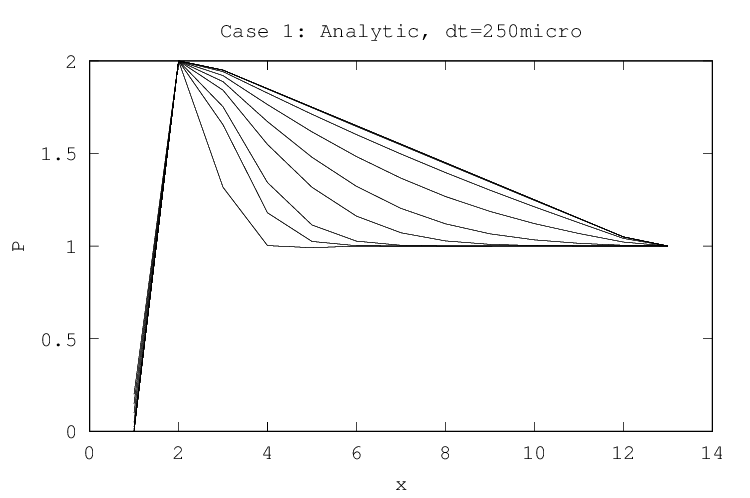
\includegraphics[]{../code/case1.png}
  \caption{Case 1.}
  \label{fig:case1}
\end{figure}

\begin{figure}[H]
  \centering
  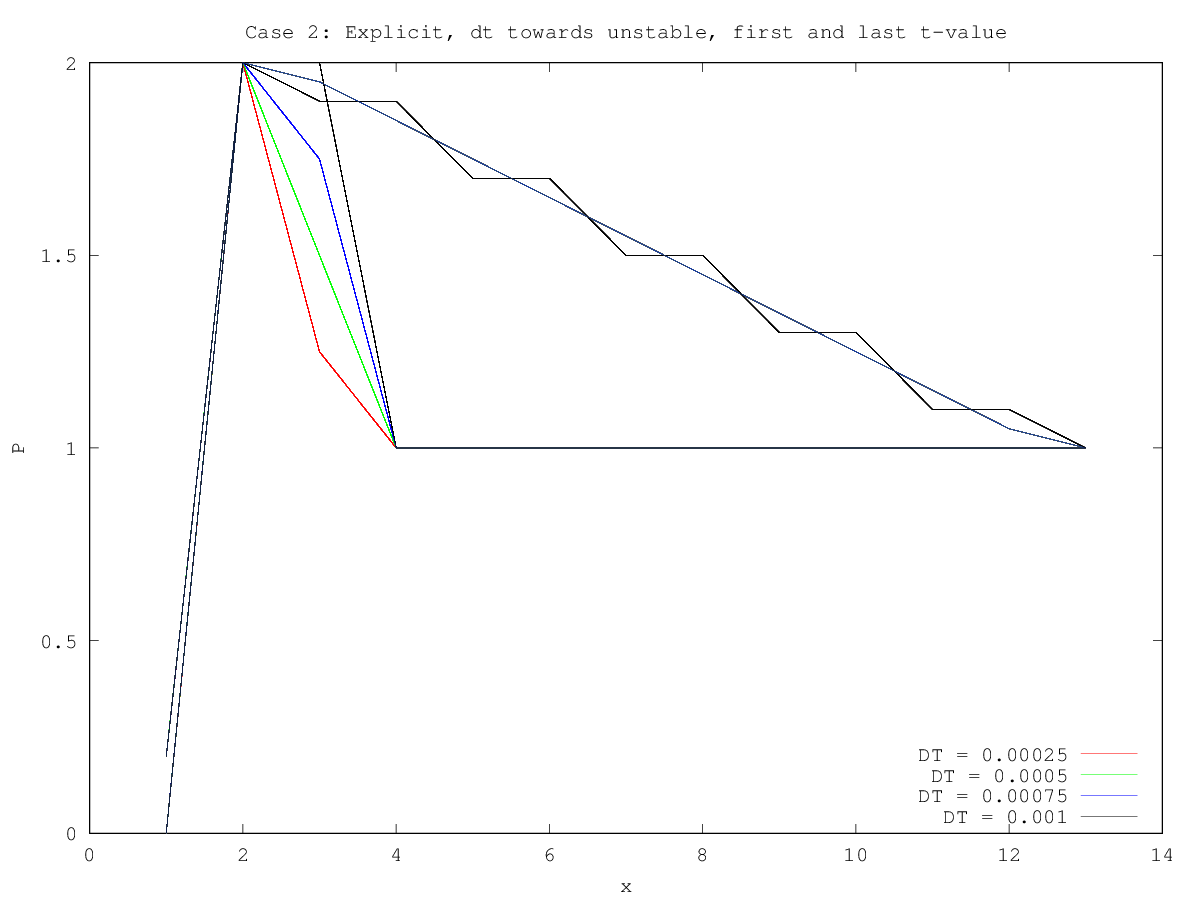
\includegraphics[]{../code/case2.png}
  \caption{Case 2.}
  \label{fig:case2}
\end{figure}

\begin{figure}[H]
  \centering
  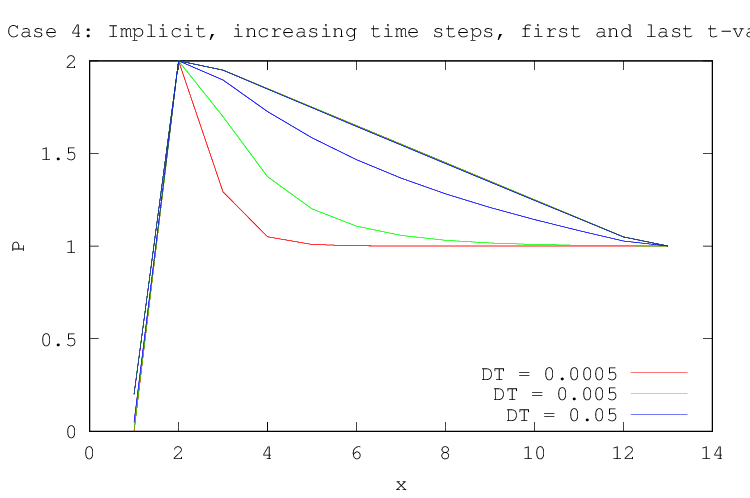
\includegraphics[]{../code/case4.png}
  \caption{Case 4.}
  \label{fig:case4}
\end{figure}

\begin{figure}[H]
  \centering
  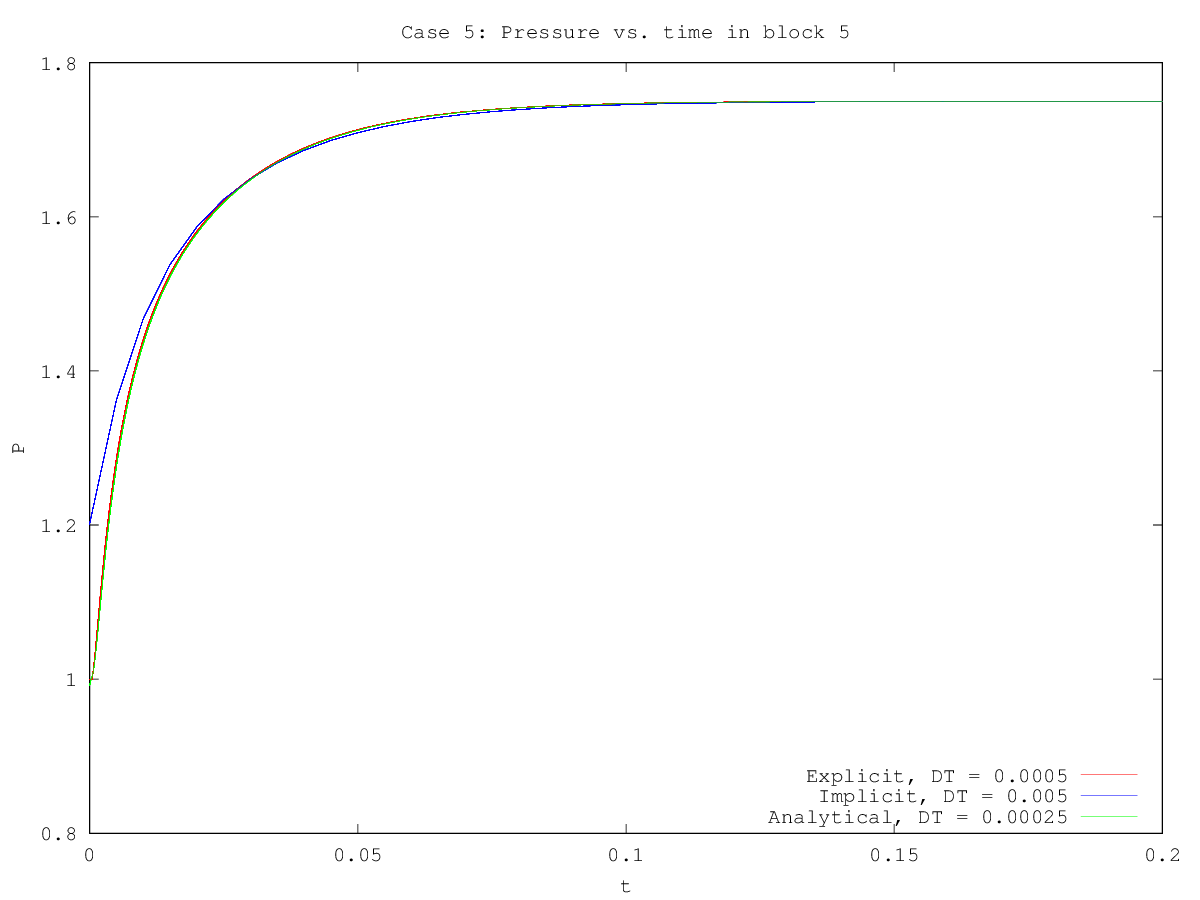
\includegraphics[]{../code/case5.png}
  \caption{Case 5.}
  \label{fig:case5}
\end{figure}

\begin{figure}[H]
  \centering
  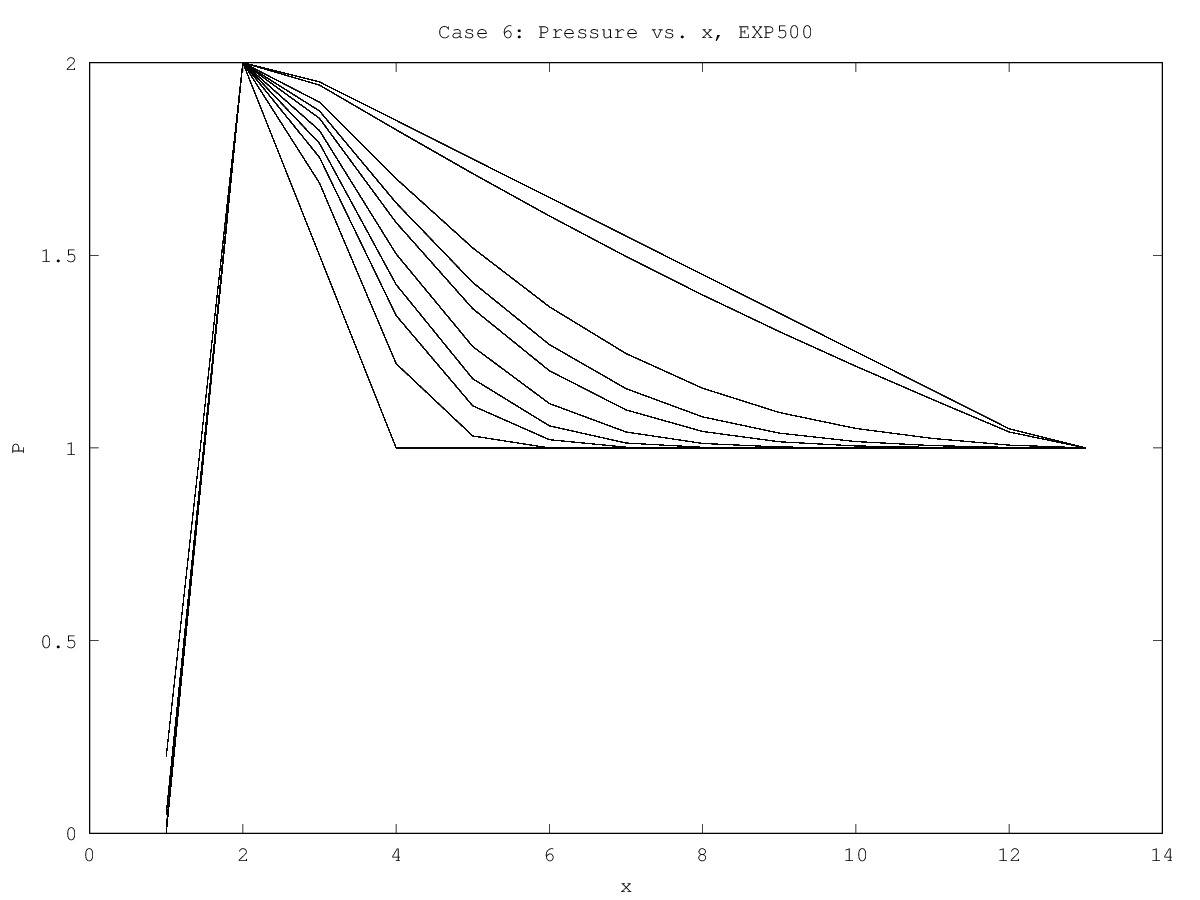
\includegraphics[]{../code/case61.png}
  \caption{Case 6, explicit solution.}
  \label{fig:case61}
\end{figure}

\begin{figure}[H]
  \centering
  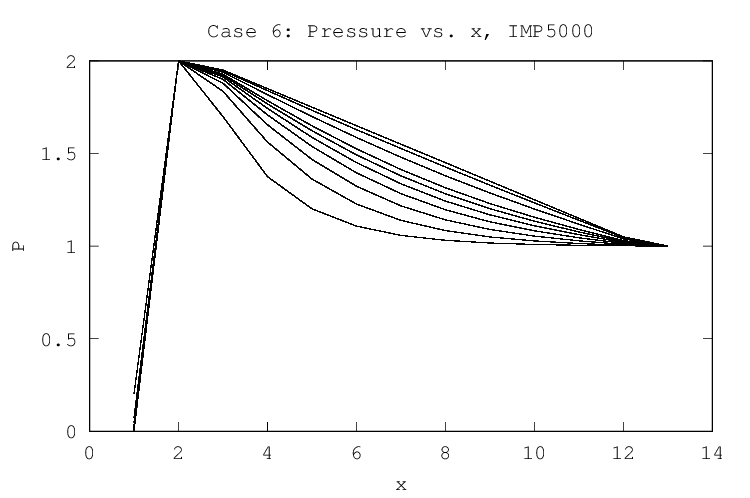
\includegraphics[]{../code/case62.png}
  \caption{Case 6, implicit solution.}
  \label{fig:case62}
\end{figure}

\begin{figure}[H]
  \centering
  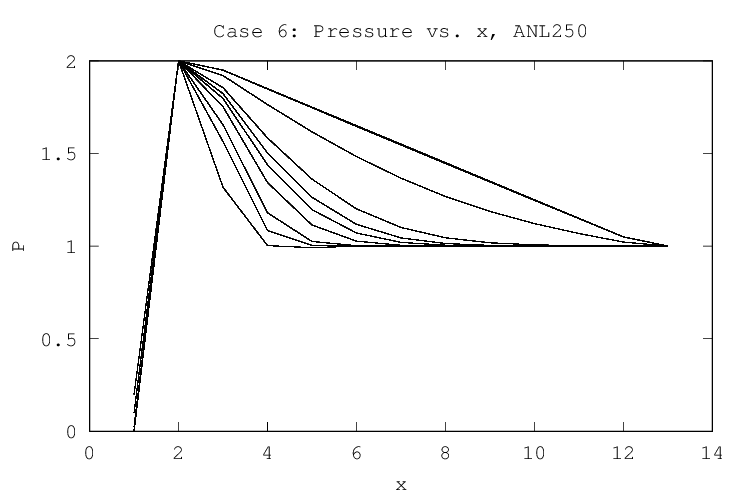
\includegraphics[]{../code/case63.png}
  \caption{Case 6, analytical solution.}
  \label{fig:case63}
\end{figure}

% subsection plots (end)
\pagebreak

\subsection{Listings} % (fold)
\label{sub:listings}

\lstinputlisting[%
  caption={Main program},
  label={lst:mainprog},
  language={[90]Fortran}]
  {../code/MainProg.f90}

\lstinputlisting[%
  caption={Shell script for data set generation},
  label={lst:shellscript},
  language={sh}]
  {../code/GenerateData.sh}

  \pagebreak

\lstinputlisting[%
  caption={Matlab script for plot generation},
  label={lst:plotgen},
  language={Matlab}]
  {../code/GeneratePlots.m}
% subsection listings (end)


% section fortran_program (end)
  
\end{document}
